\documentclass[border=4pt]{standalone}
\usepackage{amsmath,amssymb}
\usepackage{tikz}
\begin{document}
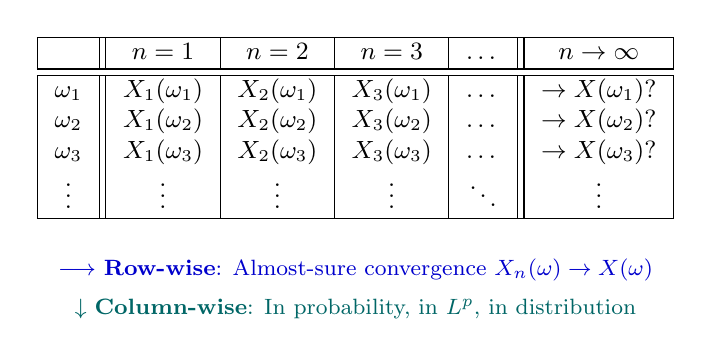
\begin{tikzpicture}[font=\small]
  \node at (0,0) {
    \begin{tabular}{|c||c|c|c|c||c|}
      \hline
      & $n=1$ & $n=2$ & $n=3$ & $\dots$ & $n \to \infty$ \\
      \hline\hline
      $\omega_1$ & $X_1(\omega_1)$ & $X_2(\omega_1)$ & $X_3(\omega_1)$ & $\dots$ & $\to X(\omega_1)$? \\
      $\omega_2$ & $X_1(\omega_2)$ & $X_2(\omega_2)$ & $X_3(\omega_2)$ & $\dots$ & $\to X(\omega_2)$? \\
      $\omega_3$ & $X_1(\omega_3)$ & $X_2(\omega_3)$ & $X_3(\omega_3)$ & $\dots$ & $\to X(\omega_3)$? \\
      $\vdots$ & $\vdots$ & $\vdots$ & $\vdots$ & $\ddots$ & $\vdots$ \\
      \hline
    \end{tabular}
  };
  \node[font=\footnotesize, text=blue!80!black] at (0, -1.8) 
    {$\longrightarrow$ \textbf{Row-wise}: Almost-sure convergence $X_n(\omega) \to X(\omega)$};
  \node[font=\footnotesize, text=teal!80!black] at (0, -2.3) 
    {$\downarrow$ \textbf{Column-wise}: In probability, in $L^p$, in distribution};
\end{tikzpicture}
\end{document}